\documentclass[11pt,a4paper]{article}

\usepackage{amsmath}  
\usepackage{amsfonts} 
\usepackage{graphicx} 
\usepackage[usenames]{color}
\usepackage{mathtools}
\usepackage{algorithm}
\usepackage{algpseudocode}
\usepackage{float}
\usepackage{xcolor}


\DeclarePairedDelimiter{\abs}{\lvert}{\rvert}
\DeclareMathOperator{\esssupp}{ess\,supp}


 \textwidth=16cm \hoffset = -1.9cm
 \lineskip=1.5\lineskip


% MATH -----------------------------------------------------------
\newcommand{\Real}{\mathbb R}
\newcommand{\eps}{\varepsilon}
\newcommand{\diag}{\mathrm{diag}}
\newcommand{\nbr}{\mathrm{nbr}}
\newcommand{\F}{\mathcal{F}}
\newcommand{\Hil}{\mathscr{H}}
\newcommand{\LL}{\mathcal{L}}
\newcommand{\G}{\mathscr{G}}
\newcommand{\s}{\mathbb{S}}
\newcommand{\p}{\mathscr{P}}
\newcommand{\C}{\mathscr{C}}
\newcommand{\one}[1]{\mathbf{1}_{\{#1\}}}
\newcommand{\oneset}[1]{\mathbf{1}_{#1}}
\renewcommand{\P}{\mathbb{P}}
\newcommand{\Q}{\mathsf{Q}}
\newcommand{\E}{\mathbb{E}}
\newcommand{\osimplex}{\mathcal{S}^{d-1}}
\newcommand{\csimplex}{\bar{\mathcal{S}}^{d-1}}
\newcommand{\argmin}{\mathrm{argmin}}
\newcommand{\argmax}{\mathrm{argmax}}
\newcommand{\var}{\mathrm{Var}}
\newcommand{\cov}{\mathrm{Cov}}
\newcommand{\ind}{\mathrm{I}}
\newcommand{\D}{\mathscr{D}}
\newcommand{\Borel}{\mathscr{B}}
\newcommand{\M}{\mathcal{M}}
\newcommand{\Z}{\mathcal{Z}}
\renewcommand{\d}[1]{\ensuremath{\operatorname{d}\!{#1}}}

\newcommand{\ben}{\begin{enumerate}}
\newcommand{\een}{\end{enumerate}}
\newcommand{\ds}{\displaystyle}

\DeclareMathOperator{\trace}{tr}
\DeclareMathOperator*{\esssup}{ess~sup}
\DeclareMathOperator*{\essinf}{ess~inf}
\DeclareMathOperator*{\diam}{diam}
\DeclareMathOperator*{\ROC}{ROC}
\DeclareMathOperator*{\sinc}{sinc}
\DeclareMathOperator*{\sign}{sign}
\newcommand{\voila}{\hfill $\blacksquare$}
\newcommand{\Id}{\mathrm{Id}}
\newcommand{\K}{\mathbb{K}}
\renewcommand{\Re}{\mathrm{Re}}
\renewcommand{\vec}[1]{\mathbf{#1}}
\newcommand*\diff{\mathop{}\!\mathrm{d}}




\title{Novel approach for modelling and forecating the spread of invasive species}


\author{Valentina Di Marco}


\date{\today}



\begin{document}
 \maketitle



\section{Hawkes Processes and Spatio-temporal self-exciting point processes}
\label{ch:Hawkes}

The idea of self-exciting point processes was first introduced by \cite{Hawkes71}. These models are well suited to events that would cluster and have been used in a variety of fields, from seismic activities (\cite{Ogata88}) to neuroscience (\cite{Reynaud}, \cite{Chornoboy}), crime prediction (\cite{Mohler13}, \cite{White} \\ \cite{Reinhart2018}) and social media (\cite{Chen}). Another interesting and application is in modelling the spread of diseases. For example \\ \cite{Browning} have recently been modelling retrospectively daily counts of deaths during the COVID-19 pandemic outbreak using a time-discrete Hawkes process. 

In our second paper, We will utilise a self-exciting spatial-temporal point process to model the RIFA invasion as in general invasive species involve clustering. This model will also allow us to disregard the phylogeny of the nests making the simulations faster than for some existing models for this invasion. The phylogeny could be reconstructed if needed.

In this chapter we aim to introduce self-exciting point process in a general manner. An in depth presentation of the subject which can be found in several books like Daily and Vere-Jones ``An Introduction to the Theory of Point Processes: Elementary Theory and Methods" (\cite{Daley}) or Snyder``Random Point Process in Time and Space" (\cite{Snyder}).

\section{Definition of a self-exciting point process}

A self-exciting point process is a counting process modelling a sequence of events over time. Each of these events will ``excite" the process, meaning that the likelihood of a new event is increased for some time after the first arrival. We will first consider the one dimensional case also known as Hawkes process.

Let us first define a counting process as a stochastic process which represents the cumulative count of the number of events in the time interval $[0, t]$. More formally

\begin{definition}
    A \textbf{counting process} is a stochastic process $(N(t) : t \geq 0)$ such that:
    \begin{enumerate}[label=(\roman*)]
        \item $N(t)$ is integer valued.
        \item If $s<t$, then $N(s) \leq N(t)$.
    \end{enumerate}
\end{definition}

This can be also viewed as a simple point process characterised by the sequence of random arrivals times $\vec{T} = \{ t_1, t_2 \dots \}$ at which the counting process has jumped. More formally (definition adapted from \cite{Jacobsen} chapter 2.1)

\begin{definition}
    A \textbf{simple point process} is a sequence of random variables $\vec{T} = \{ t_1, t_2 \dots \}$ defined on the probability space $(\Omega, \mathcal{F}, \mathbb{P})$ and with values in $\mathbb{R}_{>0} \cup \infty$ such that:
    \begin{enumerate}[label=(\roman*)]
        \item $\mathbb{P}(0 < t_0 \leq t_1 \leq \dots) = 1$.
        \item $\mathbb{P}(t_n < t_{n+1}, t_n < \infty) = \mathbb{P}(t_n < \infty)$ for $n \geq 0$.
        \item The number of random variables in a bounded region is finite almost surely (a.s.).
    \end{enumerate}
\end{definition}

Hence a simple point process is an almost surely increasing sequence of strictly positive, possibly infinite random variables, strictly increasing as long as they are finite and such that only finitely many events can occur in any finite time interval. Notice that no points coincide as they are strictly ordered in time.
The interpretation of a finite $t_n$ is the timepoint at which the $n$th recording of an event takes place with less than $n$ events occurring all together on the time axis $\mathbb{R}_{>0} \cup \infty$ if $t_n = \infty$. By definition no event can happen at time $0$. See Daley and Vere-Jones chapter 3 (\cite{Daley}) for a complete explanation on how Point processes on the line can be described.

We can characterise a point process defining the cumulative distribution function of the next arrival time conditioned on the past events $\mathcal{H}_u$

\begin{equation} \label{eq:CumDistPointProc}
    F(t|\mathcal{H}_u) = \int_u^t \mathbb{P}(t_{n+1} \in [s+\d s] | \mathcal{H}_u) \d s = \int_u^t f(s | \mathcal{H}_u) \d s
\end{equation}
were $f(s | \mathcal{H}_u)$ is the probability density function.

By the chain rule the joint density for a realisation $\{ t_1, \dots, t_k\}$ will therefore be

\begin{equation}\label{eq:JointDensHawkes}
    p(t_1, \dots, t_k) = \prod_{i=1}^k f(t_i | \mathcal{H}_{t_{i-1}}).
\end{equation}
A point process is completely defined if the joint probability distributions are known for the number of events in all finite families of disjoint intervals (see  \cite{Daley} chapter 5 and 9).

If a point process has a probability distribution function $f(t)$ that is independent of the history $\mathcal{H}_t$ we call this process a \textit{renewal process}. Another way to state this is that $f(t) = g(t - t_k)$ for some p.d.f. $g : \mathbb{R}^+ \rightarrow \mathbb{R}^+$. This way the interarrival times are independent and identically distributed (i.i.d) random variables.

An example of renewal process in which these interarrival times are exponentially distributed is the \textit{homogeneous Poisson Process}.

\begin{definition}\label{def:HomPoi}
    Consider a counting process $(N(t):t \geq 0)$ over the half-open interval $(a_i, b_i]$ with $a_i < b_i \leq a_{i+1}$, then a \textit{stationary or homogeneous Poisson Process} on the line is completely defined by
    \begin{equation}\label{001}
        \mathbb{P}(\{N(a_i, b_i] = n, i = 1, \dots, k \}) = \prod_{i=1}^k \frac{[\lambda(b_i - a_i)]^{n_i}}{n_i!}e^{-\lambda(b_i-a_i)}.
    \end{equation}
\end{definition}
Therefore for an homogeneous Poisson process the number of points in each finite interval $(a_i, b_i]$ has a Poisson distribution. Also, the number of points in disjoint intervals are independent random variables and the distributions are stationary, meaning that they depend only on the lengths of the intervals $b_i - a_i$.

The likelihood of a finite Poisson Process is the probability of obtaining the given number of observations $N$ in the observation period $(0,T]$, times the joint conditional density for the locations of those observations $t_1, \dots, t_N$, given their number. From equation (\ref{001}) we see that the probability of obtaining one event in $(t_i - \Delta, t_i]$ and no points in the remaining parts of $(0, T]$ is

\begin{equation*}
    e^{-\lambda T} \prod_{i=1}^N \lambda \Delta.
\end{equation*}
Dividing by $\Delta^N$ and letting $\Delta \rightarrow 0$ we obtain the density and therefore find the likelihood

\begin{equation*}
    L_{(0, T]}(N;t_1, \dots, t_N) = \lambda^N e^{-\lambda T}.
\end{equation*}
A Poisson process with time-varying rate $\lambda(t)$ is called \textit{inhomogeneous} Poisson process and can be defined the same way as the homogeneous Poisson process in Definition \ref{def:HomPoi} with the quantities $\lambda(b_i - a_i) = \int_{a_i}^{b_i} \lambda \d x$ replaced by

\begin{equation*}
    \Lambda(a_i, b_i] = \int_{a_i}^{b_i} \lambda(x) \d x.
\end{equation*}
The likelihood of a inhomogeneous Poisson process will then be

\begin{equation} \label{eq:LikInhPoiPro}
    L_{(0, T]}(N;t_1, \dots, t_N) = e^{-\Lambda(0, T]}\prod_{i=1}^N \lambda(t_i)
\end{equation}
and since $N$ is a counting process

\begin{equation} \label{eq:LikInhPoiPro2}
    e^{-\Lambda(0, T]}\prod_{i=1}^N \lambda(t_i) = \exp \Bigg( - \int_0^T \lambda(t)\d t + \int_0^T \log \lambda(t) N (\d t) \Bigg).
\end{equation}
Let us consider now  a time change $t \rightarrow u(t) \equiv \Lambda(0, t]$. For all $t \geq 0$ we write $N(t) = N (0, t]$ and define a new point process by $\tilde{N}(t) = N(u^{-1}(t))$. It follows that this new process has a rate quantity $\tilde{\Lambda}(0, t) = u(u^{-1}(t)) = t$ and is therefore a stationary Poisson process with $\lambda = 1$.

It can be shown that any point process that stratifies certain continuity condition can be transformed into a Poisson  process if we allow a random time change in which $\Lambda[0, t]$ depends on the past of the process up to time $t$. This result also implies that \ref{eq:LikInhPoiPro2} is the typical form of the likelihood for a point process (see \cite{Daley} chapter 2.1 and \cite{Papangelou}). 

We can now define the self-exciting Hawkes model. This model combines a cluster process representation and a simple conditional intensity representation which is moreover linear.

\begin{definition}\label{def:Hawkes}
    Let us consider a point process $N(t)$ such that
    \begin{enumerate}[label=(\roman*)]
        \item $\mathbb{P}(\{ N(t+h) - N(t) = 1 \} | \mathcal{H}_t) = \lambda(t)h + o(h)$
        \item $\mathbb{P}(\{ N(t+h) - N(t) > 1 \} | \mathcal{H}_t) = o(h)$
    \end{enumerate}
    If the quantity $\lambda(t)$ can be written as
    \begin{equation*}
        \lambda(t | \mathcal{H}_t) = \mu + \int_{0}^t g(t - u) \d N(u)
    \end{equation*}
    for some $\mu \in \mathbb{R^+}$ and $g : \mathbb{R^+} \rightarrow \mathbb{R^+} \cup \{0\}$ then this process is a \textbf{Hawkes process}.
\end{definition}
The quantity $\mu$ is called \textit{background intensity} and the function $g$ is called \textit{excitation function} of \textit{triggering function}. The quantity $\lambda(t | \mathcal{H}_t)$ representing the rate of events at time $t$ is called \textit{conditional intensity} and can be also written as

\begin{equation*}
    \lambda(t|\mathcal{H}_t) = \mu + \sum_{t_i < t} g(t - t_i)
\end{equation*}
where $\{ t_1, \dots, t_k\}$ represents the observed sequence of past events up to time $t$.

The process is called ``self-exciting" because of the dependence of the conditional intensity function on the past history $\mathcal{H}_t$ of the system allowing events to trigger new events. The triggering function $g$ can take many forms, so the process may depend only on the recent history if $g$ decays rapidly or may have longer term effects (\cite{Reinhart}). However, we generally require that $\lambda(t | \mathcal{H}_t)  \geq 0$, therefore we must have $g(t) \geq 0$ for every value of $t$ and $g(t) = 0$ for $t < 0$.

The general definition for the conditional intensity $\lambda$ for any point process is

\begin{equation*}
    \lambda(t | \mathcal{H}_t) = \lim_{h \to 0} \frac{\mathbb{E}[N(t+h) - N(t) | \mathcal{H}_t]}{h}
\end{equation*}
so it represents the mean number of events in a region conditional on the past.
Let us rewrite this last equation (\cite{Rasmussen})

\begin{equation*}
    \lambda(t | \mathcal{H}_t) \d t = \mathbb{E}[N(\d t) | \mathcal{H}_t]
\end{equation*}
were $\d t$ is an infinitesimal interval around $t$.
The intensity function will therefore be:

\begin{align*}
    \mathbb{E}[N(\d t) | \mathcal{H}_t] &= \mathbb{P}(\textrm{point in} \d t | \mathcal{H}_t) \\
    & = \mathbb{P}(\textrm{point in} \d t | \textrm{point not before } t, \mathcal{H}_t) \\
    & = \frac{\mathbb{P}(\textrm{point in} \d t, \textrm{point not before } t | \mathcal{H}_t)}{\mathbb{P}(\textrm{point not before } t | \mathcal{H}_t))} \\
    & = \frac{\mathbb{P}(\textrm{point in} \d t | \mathcal{H}_t)}{\mathbb{P}(\textrm{point not before } t | \mathcal{H}_t))} \\
    & = \frac{f(t) \d t}{1 - F(t)}
\end{align*}
Where the quantities $f(t)$ and $F(t)$ where defined in equation (\ref{eq:CumDistPointProc}). So the intensity function can be written
\begin{equation}\label{eq:IntFun}
    \lambda(t) = \frac{f(t) \d t}{1 - F(t)}.
\end{equation}
For ease of notation here and from now on we are omitting the conditioning over the past events $\mathcal{H}_t$.


\begin{figure*}
\centering
    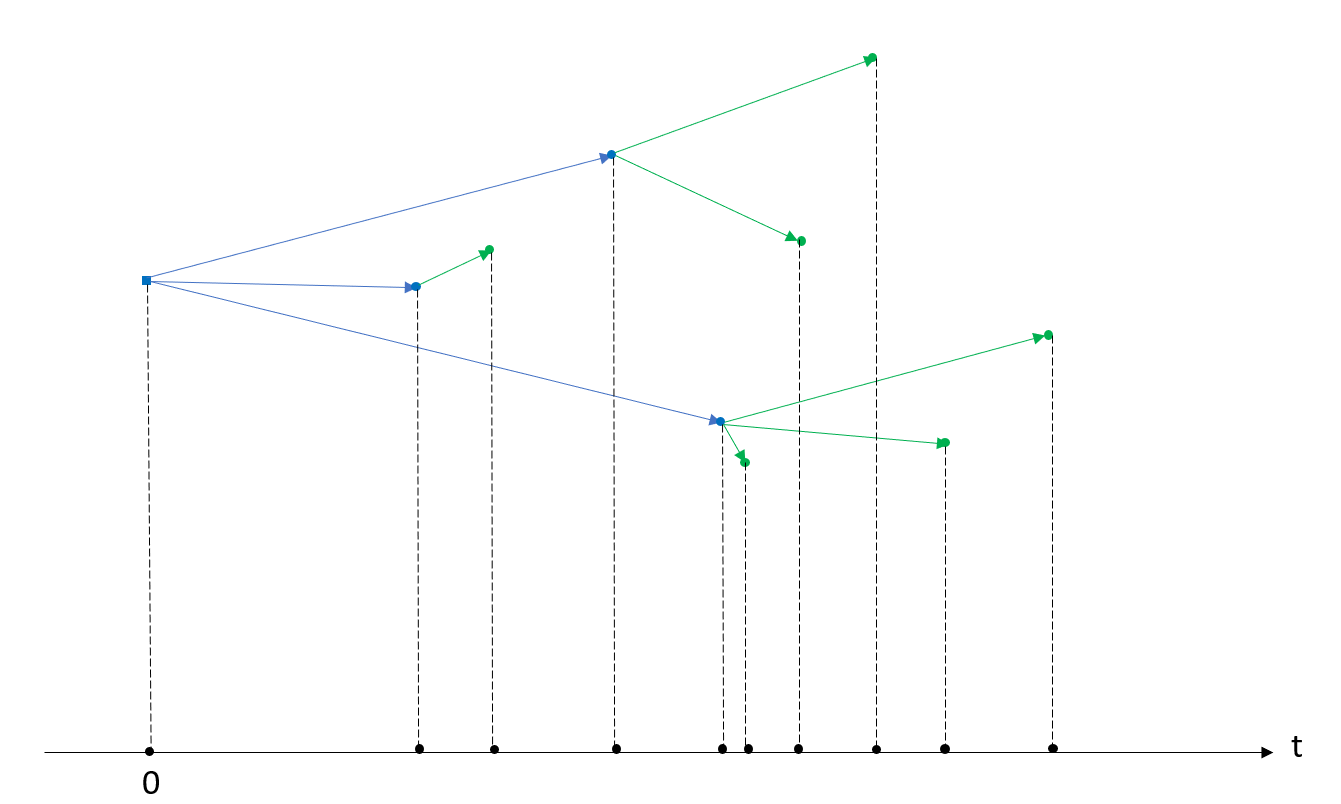
\includegraphics[width=0.8\linewidth]{Hawkes.PNG}
\caption{Branching structure (immigration-birth representation) for the cluster generated by one immigrant (blue square). The blue circles represent the first generation and the green circles the second generation. The black dots on the timeline denote the generated point process.}
\label{fig:Hawkes}
\end{figure*}







\section{Immigration-birth representation} \label{ch:immi}

A Poisson cluster process $\bm{X} \subset \mathbb{R}$ is a Point process in which the cluster centers of $\bm{X}$ are given by points called immigrants and the other points of the process are called offspring. It is defined as follow (\cite{Bordenave}):
\begin{itemize}
    \item Immigrants are distributed according to a homogeneous Poisson process $I$ with points $X_i \in \mathbb{R}$ and intensity $\mu > 0$.
    \item Each immigrant $X_i$ generates a cluster $C_i = C_{X_i}$, which has a finite number of points almost surely.
    \item Given the immigrants, the centered clusters 
    \begin{equation*}
        C_i - X_i = \{Y - X_i: Y \in C_i\}, \quad X_i \in I
    \end{equation*}
    are i.i.d. and independent of $I$.
    \item $\bm{X}$ consists of the union of all the clusters.
\end{itemize}

We call $S$ the number of points in a cluster and assume that the expectation $\mathbb{E}[S] < \infty$. If $\bm{Y}$ is a point process in $\mathbb{R}$ and $N_{\bm{Y}}(0, t]$ is the number of points of this process in the interval $(0, t]$, then $\bm{Y}$ is stationary if its law is translation invariant and it is ergodic if it is stationary with a finite intensity $\mathbb{E}[N_{\bm{Y}}(0, 1]]$ and

\begin{equation*}
    \lim_{t \rightarrow \infty} \frac{N_{\bm{Y}}(0, t]}{t} = \mathbb{E}[N_{\bm{Y}}(0, 1]], \quad \text{a.s.}
\end{equation*}
It follows then that the Poisson cluster process defined above is ergodic with finite intensity $\mu \mathbb{E}[S]$ and

\begin{equation*}
    \lim_{t \rightarrow \infty} \frac{N_{\bm{X}}(0, t]}{t} = \nu\mathbb{E}[S], \quad \text{a.s.}
\end{equation*}

It has been proved by \cite{Hawkes74} that any stationary self-exciting point process with finite intensity function can be interpreted as a Poisson cluster process. In this process each immigrant $X_i$ generates a cluster $C_i = C_{X_i}$, which is the random set formed by the points of generation $n = 0, 1, \dots$ with the following branching structure: the immigrant $X_i$ is said to be of generation $0$. Given generations $0, 1, \dots, n$ in the cluster $C_i$, each point $Y \in C_i$ of generation $n$ generates a Poisson process on $(Y, \infty)$, say $\Phi$, of offspring of generation $n+1$ with intensity function $g(\cdot - Y)$. Here $g:(0, \infty) \rightarrow [0, \infty)$ is a non-negative Borel function.

The mean number of points in any offspring process $\Phi$ is

\begin{equation*}
    m = \int_0^\infty g(t) \d t
\end{equation*}
with $0 < m < 1$.
The condition $m > 0$ excludes the trivial case in which there are almost surerely no offspring.
\cite{Hawkes74} noted that the total number of points in a cluster process is equivalent to the total progeny of a Galton-Watson process with one ancestor and number of offspring per individual following a Poisson distribution with mean $m$. Therefore the condition $m < 1$ is equivalent to assuming that $\mathbb{E}[S] = 1/(1 - m) < \infty$.

From theorem 2.11.2 in \cite{Jagers} it follows that

\begin{equation*}
    p(S = k) = \frac{e^{km}(km)^{k-1}}{k!}, \quad k = 1, 2, \dots
\end{equation*}
Finally, since $\bm{X}$ is ergodic with a finite and positive intensity equal to $\mu/(1 - m)$ it holds that

\begin{equation*}
    \lim_{t \rightarrow \infty}\frac{N_{\bm{X}}(0, t]}{t} = \frac{\nu}{(1 - m)} \quad \text{a.s.}
\end{equation*}






\section{self-exciting spatial-temporal point process}

So far we have considered only the temporal form of the self-exciting point processes but we can extend this models to spatio-temporal processes. The definition will be analogous to Definition \ref{def:Hawkes} with conditional intensity

\begin{equation*}
    \lambda(s, t) = \mu(s) + \sum_{i:t_i<t} g(s - s_i, t - t_i),
\end{equation*}
where $\{ s_1, \dots, s_n \}$ are the observed locations of events and $\{t_1, \dots t_n \}$ the observed times of events. 

Similarly to the Hawkes' self-exciting temporal processes, the self-exciting spatio-temporal point processes can be treated as Poisson cluster processes with the locations of events $s \in X \subseteq \mathbb{R}^d$ and times $t \in (0, T]$. The mean number of offspring will be

\begin{equation}\label{eq:meanoffsp}
    m = \int_X \int_0^T g(s, t) \d t \d s.
\end{equation}
We have considered the points of a point process as indistinguishable other then by their time and location. Often, however, we need to take in consideration other quantities. For example, one may wish to analyse locations and time of observations of an invasive species plant alongside the age of the organism. Such process may be viewed as a \textit{marked} point process. A marked point process is a point process of events $\{ (s_i, t_i, k_i ) \}$ where  $s_i \in X \subseteq \mathbb{R^d}$, $t_i \in [0, T)$ and $k_i \in \mathcal{K}$ where $K$ is the \textit{marked space} (in our example the space of plants ages).

The \textit{ground process} of a marked point process is the point process of events locations and times without the marks with conditional intensity $\lambda_g(s, t)$. The conditional intensity for the marked point process can be written as

\begin{equation*}
    \lambda(s, t, k) = \lambda_g(s, t)f(k | s, t),
\end{equation*}
where $f(k | s, t)$ is the conditional density of the mark at time $t$ and location $s$ given the history of the process up to time $t$.








\section{The likelihood of a self-exciting point process}

We obtain the Likelihood for a Hawkes process from the following theorem

\begin{theorem}
    Let $N(\cdot)$ be a regular point process on [0, T] for some positive T, and let $\{ t_1, \dots, t_k \}$ denote the realisation of $N(\cdot)$ over [0, T]. Then, the likelihood $L$ of $N(\cdot)$ is expressible in the form
    \begin{equation*}
        L = \Bigg [ \prod_{i=1}^k \lambda(t_i) \Bigg] exp \Bigg( - \int_0^T \lambda(u) \d u \Bigg).
    \end{equation*}
\end{theorem}

\begin{proof}
    From equation \ref{eq:JointDensHawkes} the joint density function is
    
    \begin{equation*}
        L = p(t_1, \dots, t_k) = \prod_{i = 1}^k f(t_i).
    \end{equation*}
    From equation (\ref{eq:IntFun}) we have
    
    \begin{equation*}
        \lambda(t) = \frac{f(t)}{1 - F(t)} = \frac{\frac{\mathrm{d} F(t)}{\mathrm{d} t}}{1 - F(t)} = - \frac{\mathrm{d}}{\mathrm{d} t} \log(1 - F(t))
    \end{equation*}
    therefore integrating both sides over the interval $(t_k, t)$ we have
    
    \begin{equation*}
        \int_{t_k}^t \lambda (u) \d u = - [\log(1 - F(t)) - \log(1 - F(t_k))].
    \end{equation*}
    Since the Hawkes process is a simple process, multiple arrivals cannot occur and $F(t_k) = 0$ as the probability that point $t_{k+1}$ falls on top of $t_k$ is zero, therefore we have
    
    \begin{equation}\label{logCDF}
        \int_{t_k}^t \lambda (u) \d u = - \log(1 - F(t)).
    \end{equation}
    Rearranging we have
    
    \begin{align*}
        & F(t) = 1 - \exp \Bigg( -\int_{t_k}^t \lambda(u) \d u \Bigg) \\
        & f(t) = \lambda(t) \exp \Bigg( -\int_{t_k}^t \lambda(u) \d u \Bigg)
    \end{align*}
    and the likelihood for observing a process until the time of the $k$th arrival becomes
    
    \begin{align*}
        L &= \prod_{i=1}^k f(t_i) \\
        &= \prod_{i=1}^k \lambda(t_i) \exp \Bigg( -\int_{t_{i-1}}^{t_i} \lambda(u) \d u \Bigg) \\
        &= \Bigg[ \prod_{i=1}^k \lambda(t_i) \Bigg]\exp \Bigg( -\int_{0}^{t_k} \lambda(u) \d u \Bigg).
    \end{align*}
    When a process is observed over a time period $[0, T] \subset [0, t_k]$ we will need to include in the likelihood the probability of seeing no arrivals in the interval $(t_k, T]$ so the likelihood becomes:
    
    \begin{equation*}
        L = \Bigg[ \prod_{i=1}^k f(t_i) \Bigg] (1 - F(T)) = \Bigg[ \prod_{i=1}^k \lambda(t_i) \Bigg]\exp \Bigg( -\int_{0}^{T} \lambda(u) \d u \Bigg).
    \end{equation*}
\end{proof}
Notice that this is the likelihood of an inhomogeneous Poisson process with $\Lambda(0, T] = -\int_{0}^T \lambda(u) \d u$ as in equation (\ref{eq:LikInhPoiPro}).

The likelihood for a temporal point process can also be defined in terms of the Janossy density. Here we only make a quick mention of the method. For a full explanation see Daley Chapter 7 (\cite{Daley})).
Let $(A_1, \dots, A_k)$ be a partition of $[0, T]$ with $A_i$ the possible times for event $i$ and let us call $p_k$ with $k = 0, 1, \dots$ the distribution of the total number of points, with $\sum_{k=0}^\infty p_k = 1$. Let us also define for each integer $k \geq 1$ the probability distribution $\Pi_k^{sym}(\cdot)$ determining the joint distribution of the times of events in the process, given there are $k$ total events. This distribution is symmetric because we consider unordered sets and this distribution should therefore give equal weights to all $k!$. We define the Janossy measure $J_k$ as
\begin{equation*}
    J_k(A_1 \times \dots \times A_k) = k!p_k\Pi_k^{sym}(A_1 \times \dots \times A_k).
\end{equation*}
Notice that the Janossy measure is not a probability measure, but it represents the sum of the probabilities of all $k!$ permutations of $k$ points. 
When derivatives exists we can introduce the density $j_k(t_1, \dots, t_k)$ of the Janossy measure with respect to the Lebesgue measure on $(\mathbb{R})^k$ with $t_i \neq t_j$ for $i \neq j$. Then the quantity $j_n(t_1, \dots, t_n)\d t_1, \dots \d t_n$ can be interpreted as the probability that there are exactly $n$ events in the process, one in each of the infinitesimal intervals $(t_i, t_i+\d t_i)$. This interpretation connects the Janossy density to the likelihood function which can be written
\begin{equation*}
    L(t_i,\dots, t_k) = j_k(t_1, \dots, t_k | T)
\end{equation*}
were $j_k(t_1, \dots, t_k | T)$ is the local Janossy density interpreted as the probability that there are exactly $k$ events in the process before time $T$, one in each of the infinitesimal intervals.

The likelihood of a spatio-temporal self-exciting point process is obtained by treating the spatial locations as marks therefore obtain the log-likelihood (Daley and Vere-Jones (2003) Proposition 7.3.III) (\cite{Daley})

\begin{proposition}
    Let $N$ be a regular marked point process on $[0, T] \times X$ where $X \subset \mathbb{R}^2$ for some positive $T$, and let $(t_1, x_1), \dots, (t_{N_g(T)}, x_{N_g(T)})$ be a realisation of $N$ over the interval $[0, T]$. Then the likelihood $L$ of such a realisation is expressible  in the form
    
    \begin{align*}
        L &= \Bigg[ \prod_{i=1}^{N_g(T)} \lambda(t_i, x_i) \Bigg]\exp \Bigg( -\int_{0}^{T} \int_X \lambda(u, k) \d u \d k \Bigg) \\
        &= \Bigg[ \prod_{i=1}^{N_g(T)} \lambda_g(t_i) \Bigg] \Bigg[ \prod_{i=1}^{N_g(T)} f(x_i | t_i) \Bigg]\exp \Bigg( -\int_{0}^{T} \lambda_g(u) \d u \Bigg)
    \end{align*}
\end{proposition}
were $\lambda_g(t)$ is the ground process and $f(x | t)$ is the conditional probability of the marks 

\begin{equation*}
    l = \sum_{i=1}^n log(\lambda(s_i, t_i)) - \int_0^T\int_X \lambda(s,t) \d s \d t
\end{equation*}







\section{Simulation of self-exciting point processes}

The simulation of a Hawkes is a similar problem to the simulation of a inhomogeneous Poisson process which is achieved via thinning. For a inhomogeneous Poisson process with time-varying intensity $\lambda(\cdot)$ the thinning procedure is intuitively done generating a ``faster" homogeneous Poisson process, then removing points in a probabilistic way. The remaining points will then satisfy the intensity $\lambda(\cdot)$. The rate of the first process cannot be less than $\lambda(\cdot)$ over $[0, T]$. Formally the process is described by \cite{Lewis}.

\cite{Ogata81} introduced a simulation algorithm for point processes which is based on the thinning algorithm for inhomogeneous Poisson processes. To apply this method to an Hawkes process we notice that while the intensity for this process does not have an almost surely upper bound, it is common for the intensity to be non-increasing in periods without any arrivals. In this case for $t \in [T_i, T_{i+1}]$ we have $\lambda(t) \leq \lambda (T^+_i)$ where with $T^+_i$ we mean the time just after $T_i$ when that arrival has been registered. So the value of the ``faster" process rate can be updated at each simulation.

Algorithm (\ref{Thinning}) (\cite{Laub}) describes the the thinning process 


\begin{algorithm}[H]
    \caption{Ogata's modified thinning algorithm $(T, \lambda(\cdot))$}\label{Thinning}
    \begin{algorithmic}
        \Require
            \Statex $\lambda(\cdot)$ non-increasing in periods of no arrivals.
            \Statex $\varepsilon \gets 10^{-10}$ (a small positive value).
            \Statex $P \gets []$, $t \gets 0$.
        \While{$t < T$}
            \State Find new upper bound: $M \gets \lambda(t + \epsilon)$.
            \State Generate next candidate point: $E \gets \exp(M)$, $t \gets t + E$.
            \State Keep it with probability $U \gets$ Unif $(0, M)$.
            \If {$t < 1 $ and $U \leq \lambda(t)$}
                \State $P \gets [P, t]$.
            \EndIf
        \EndWhile
        \State \Return{$P$}
    \end{algorithmic}
\end{algorithm}


The immigration-birth representation described in chapter \ref{ch:immi} gives rise to another simulation procedure which here we will call cluster algorithm. This is a simpler and faster procedure compared to the thinning algorithm as it does not require the repeated evaluation of $\lambda(\cdot)$.

As we have seen in chapter \ref{ch:immi}, the immigrants form a homogeneous Poisson process with rate $\mu$, so the number of immigrants over an interval $[0, T]$ is $\text{Pois}(\mu T)$. The arrival times of these immigrants conditional on the number of immigrants $k$ are distributed as the order statistics from a uniform distribution supported on $[0, T]$. We will call the arrival times $C_1, \dots, C_k$.

We have also seen in chapter \ref{ch:immi} that the offspring of each immigrant form an inhomogeneous Poisson process. The $i$th immmigrant's descendants will therefore arrive with intensity $\lambda(t-C_i)$ for $t > C_i$. The number of offspring of the immigrant $i$ will be denoted by $D_i$ and will be such that $D_i \overset{iid}{\sim}\text{Poi}(m)$ where $m$ has been defined in equation (\ref{eq:meanoffsp}). Say the offspring of the $i$th immigrant arrive at time $(C_i + E_1, C_i + E_2, \dots, C_i + E_{D_i})$. Conditioned on knowing $D_i$, $E_j$ are i.i.d. random variables distributed with p.d.f. $g(\cdot)/m$.


Algorithm (\ref{Cluster}) (\cite{Laub}) describes the the cluster process.


\begin{algorithm}[H]
    \caption{cluster algorithm $(T, \lambda(\cdot), m)$}\label{Cluster}
    \begin{algorithmic}
        \Statex $P \gets []$.
        \Statex Immigrants: $k \gets$ Poi$(\mu T)$, $C_1, C_2, \dots, C_k \stackrel{iid}{\gets}$ Unif$(0,T)$.
        \Statex Descendants: $D_1, D_2, \dots, D_k \stackrel{iid}{\gets}$ Poi$(m)$.
        \For{$i \gets 1$ \bf{to} $k$}
            \If {$D_i > 0$}
                \State $E_1, E_2, \dots, E_{D_i} \stackrel{iid}{\gets} g(\cdot)/m$
                \State $P \gets P \cup \{ C_i + E_1, C_i + E_2, \dots, C_i + E_{D_i}\}$
            \EndIf
        \EndFor
        \Statex Remove descendants outside $[0,T]$:
        \Statex Add in immigrants and sort: $P \gets(P \cup \{ P_i:P-i \inP, P_i \leq T \})$
        \State \Return{$P$}
    \end{algorithmic}
\end{algorithm}

Other simulations methods are available for self-exciting point processes. For example the transformation method arises from the converse of the random time \cite{Laub}. However this method can require significant computational effort and it is mostly used when the intensity function is exponentially decaying. 

For temporal point processes, a range of simulation methods are described by \cite{Daley} (section 7.5).

A Simulation process based on the branching structure of a self-exciting spatial-temporal point process was introduced by \cite{Zhuang}. 

\cite{Moller} developed a perfect simulation algorithm for temporal Hawkes processes which avoids edge effects, but its extension to spatio-temporal processes remains to be developed \cite{Reinhart}.

In our paper on the reconstruction of the fire ants invasion (chapter \ref{ch:ModelMethod}) we will utilise the cluster algorithm modified for a spatial-temporal point process.



\end{document}
